\begin{figure}
    \begin{center}
    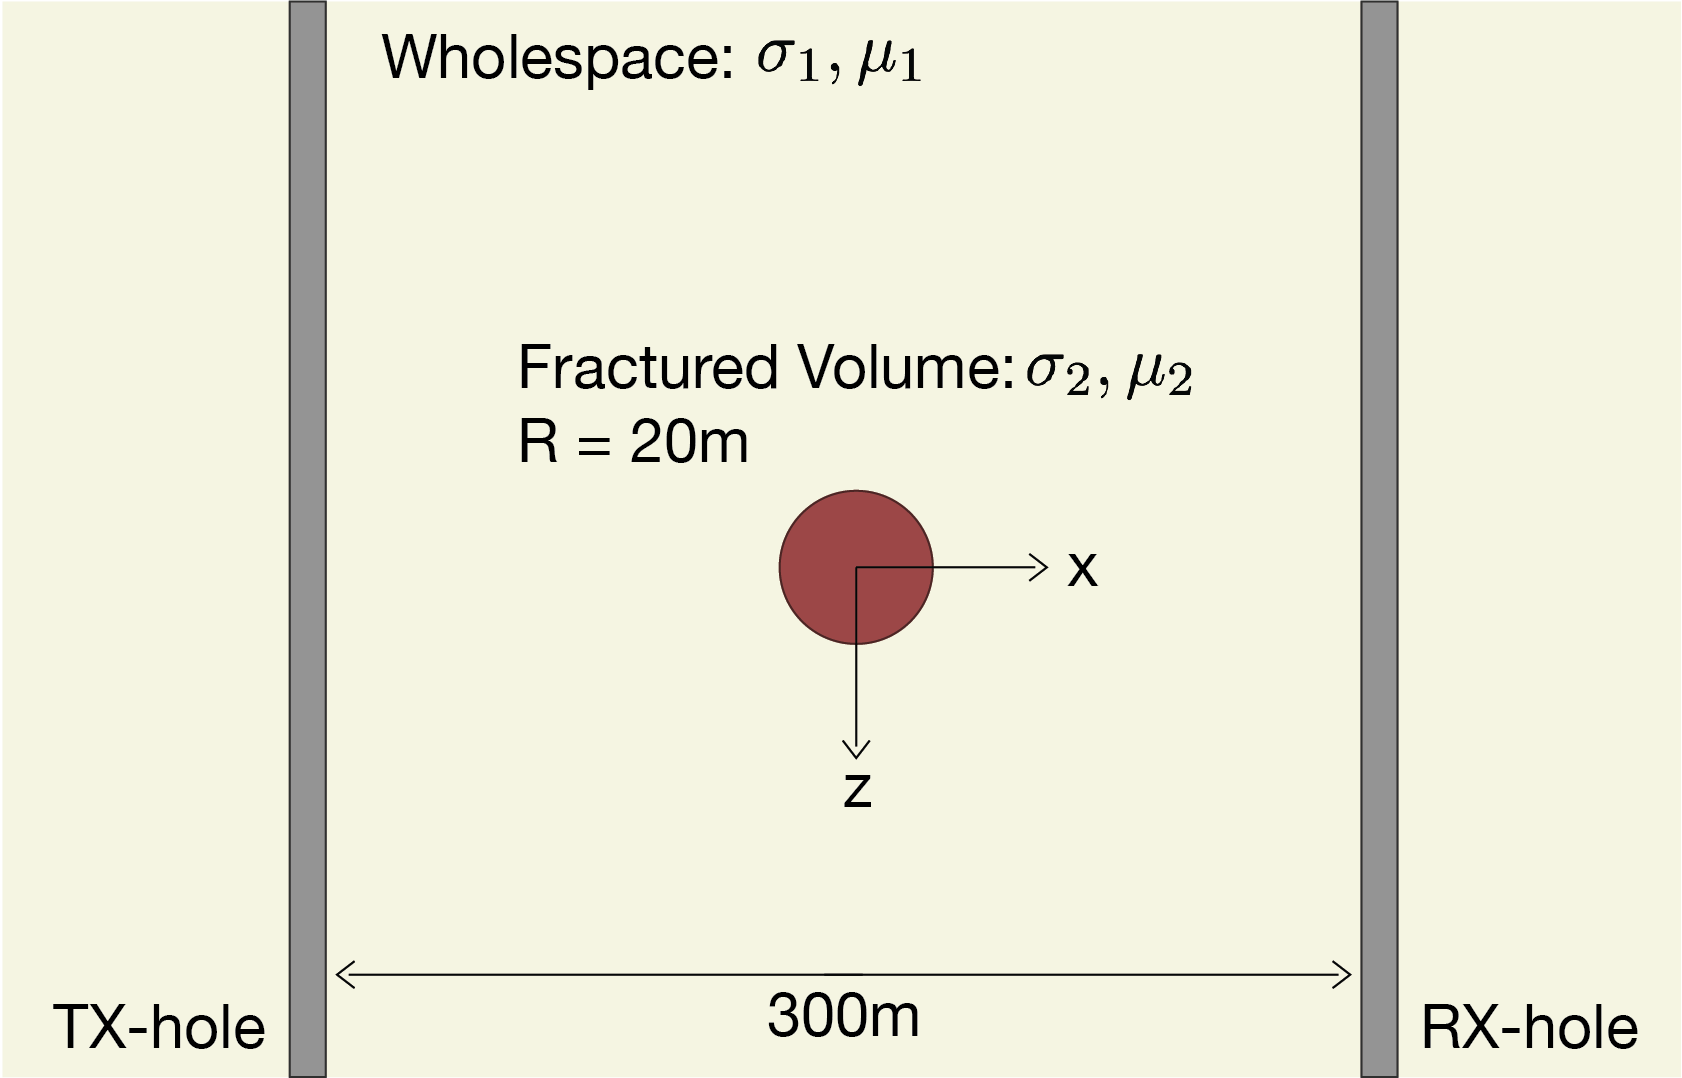
\includegraphics[width=\columnwidth]{figures/phys_prop_model/sphere_frac.png}
    \end{center}
\caption{
    Representative model of a cross-well experiment aimed at detecting
    fractured volume of rock. The fractured rock volume is approximated as a sphere
    with 20m radius, conductivity $\sigma_2$, permeability $\mu_2$, that is
    positioned mid-way between the transmitter and receiver wells. The background
    is a whole-space with conductivity $\sigma_1$ and permeability $\mu_1$
}
\label{fig:sphere_frac}
\end{figure}
